\chapter{Use cases, requirements and system overview}
\label{cha:solution-overview}
This chapter starts by introducing three use cases that illustrate the problem statement. To illustrate the problems that occur in these use cases more clearly, a generic data aggregation architecture is subsequently presented. This architecture will highlight a number of problems that currently exist and, together with the use cases, will serve to derive a number of 
requirements and an adversary model.

Thereupon, based on all these requirements, a high-level overview of the middleware system is given. This middleware, called the Middleware for Aggregation Security in Solid (MASS), is partially implemented as a prototype on top op the \acrlong{CSS}. The next chapters
then starts by studying a number of \gls{PETs} in order to determine which technologies are usable in \middleware{}. The chapters following this finally discuss the components of the solution in detail.

\section{Use cases: health and finance}
\label{sec:usecases}
This section describes three use cases which highlight the need for a middleware for secure and protected data aggregation in Solid. These use cases illustrate the complexities and challenges that come with developing such a middleware, and will serve as a guide throughout the development of the solution. The use cases are located in the domains of health and finance, since these traditionally come with sensitive data. Furthermore, data in these domains can also lead to interesting insights, forming ideal candidates for data aggregation.

\subsection{Exercise data}
\label{usecase:ex-data}
In this use case a user stores her exercise data from an application such as Strava\footnote{An application for tracking running and cycling sessions, see \url{https://www.strava.com}} on her Solid pod. She wishes to export this data to a ranking board application to see which of her friends runs the fastest. However, she does not wish to share her exact heart rate since this is sensitive data and might leak information about her fitness. This data is stored in the TCX file format\footnote{Schema: \url{https://www8.garmin.com/xmlschemas/TrainingCenterDatabasev2.xsd}}. An advantage of this format is that it is supported by popular tools such as Strava and can be imported/exported by exercise trackers such as Garmin devices.

\subsection{Personal finance}
\label{usecase:personal-finance}
This use case describes a scenario wherein a user has stored all his transactions on his Solid pod. He wishes to see some trends and statistics about his spending, and compare this to similar households. An example of such a statistic is ``how much do I spend on groceries every week?''.  However, expenses are very sensitive data, especially when these are exact numbers and store locations. Therefore, the middleware should filter out the most sensitive information while still keeping enough data to generate relevant statistics. This can be done, for example, by removing direct identifiers and perturbing exact spending at individual transactions. For example, for entries of the type ``Bob spent \texteuro 5,82 at Colruyt Leuven on 8/11/2021 16:53'', the user wishes that this is modified into something similar to ``User87532 spent \texteuro 5 at Supermarket on 8/11/2021''. This way, trends in the spending are kept (by perturbing exact amounts to nearby integers, and replacing exact stores with store types). Information such as ``you spent \texteuro 400 in supermarkets this month'' will still be available (and relatively accurate), without giving away exact details. For this use case a custom data format is used, since most standard data schemes for financial information are overly complex for a proof-of-concept.

\subsection{Aggregated view on personal health data streams}
The third use case is taken from one of the SolidLab\footnote{A research project initiated by the Flemish government \citepjournal{solid-flanders}} challenges. Concretely, the challenge \textit{aggregated view on sensitive personal health data streams} is studied\footnote{See \url{https://github.com/SolidLabResearch/Challenges/issues/16}}.

This use case describes a scenario wherein a caretaker wishes to gain insights on all her patients, without knowing exact patient details. These insights are provided through a dashboard, which shows some key statistics about the patient population. Examples of such statistics are average heart rates, average number of steps taken throughout the day, what percentage of the population woke up before 9 am, etc. Of course, the collection and aggregation of such data does not come without issues. Data is derived from activity trackers and IoT sensors, which regularly update data in the user's pod. A secure aggregator must then collect data from all these pods, combine these into aggregate statistics, and write this to a new pod accessible to the caretaker.

\newpage

\section{A generic data aggregation architecture in Solid}
\label{sec:generic-agg-arch}
All of the above use cases make use of an aggregation system that collects sensitive data and displays an aggregated view of some kind. Such an aggregation system in Solid will necessarily consist of a number of components, each with their own responsibility. Figure \ref{fig:reference-architecture} illustrates a reference architecture of such a system in Solid. 

\begin{figure}[h]
    \centering
    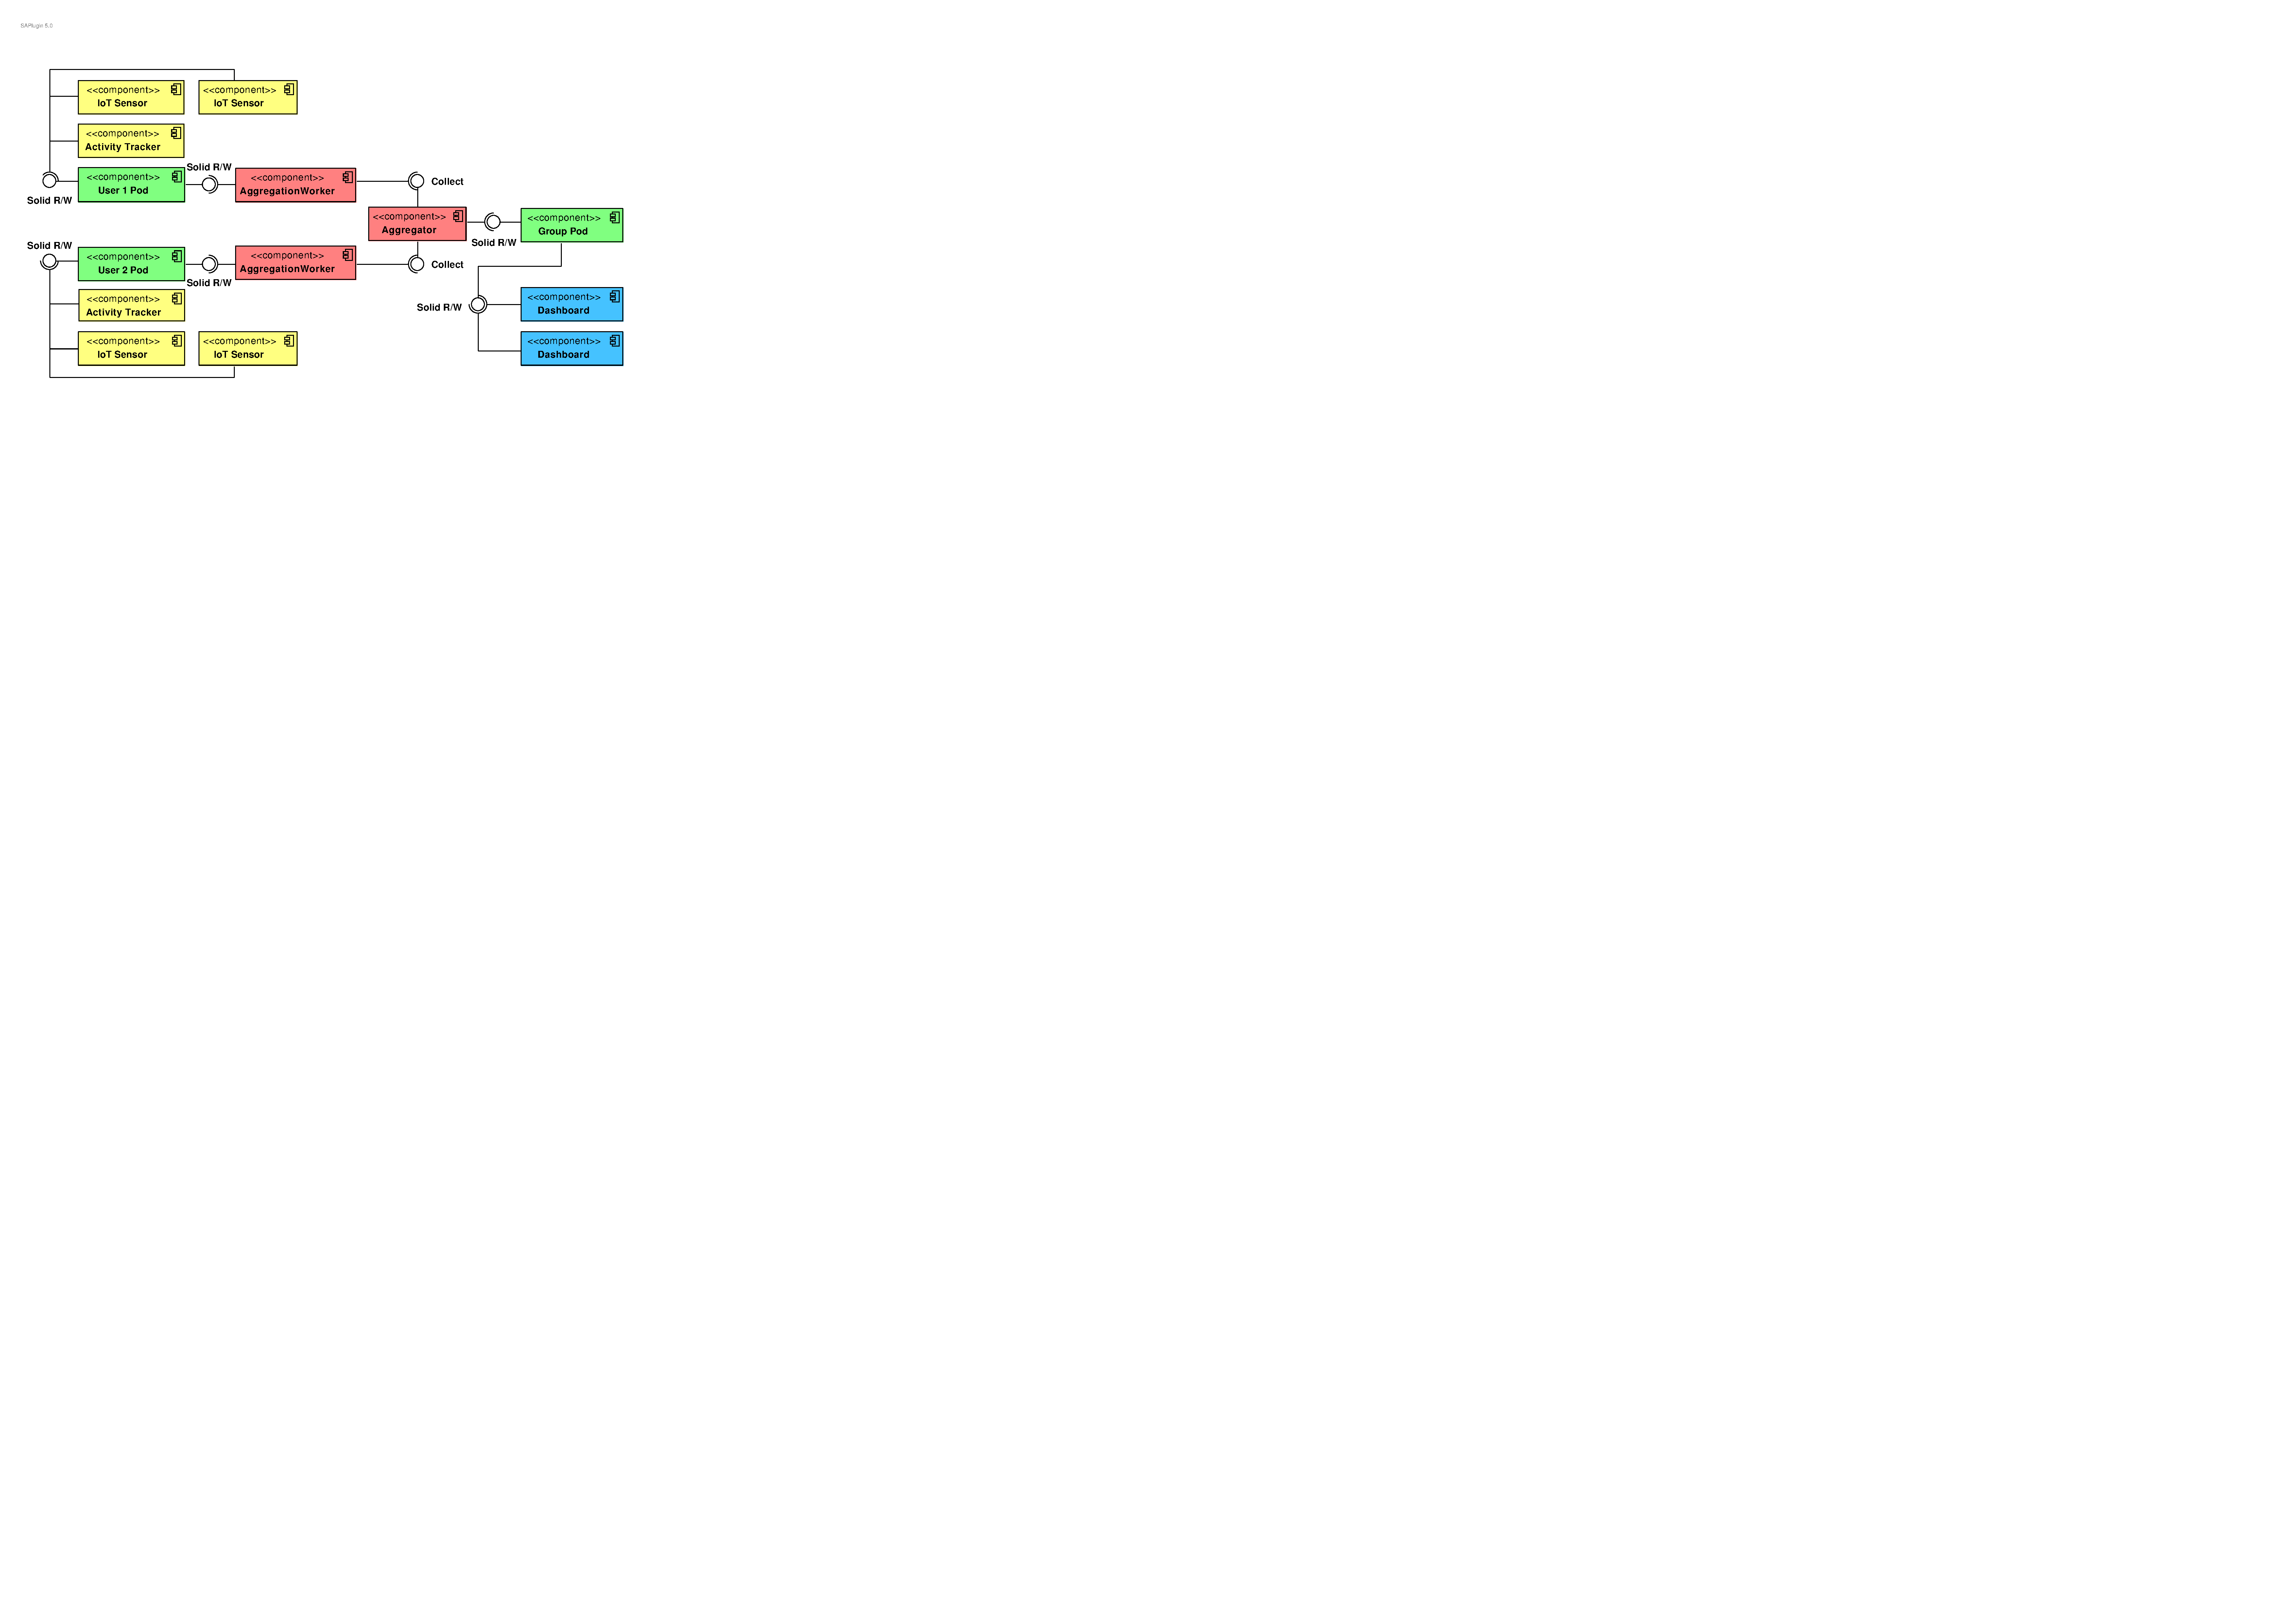
\includegraphics[width=1.0\textwidth]{images/architecture/Reference-Architecture-Aggregator.pdf}
    \caption{Reference architecture for data aggregation in Solid}
    \label{fig:reference-architecture}
\end{figure}

\noindent This reference architecture highlights a number of challenges that make aggregation insecure, unscalable, or privacy-invasive. Concretely, the following issues are remarked:

\begin{enumerate}
    \item IoT Sensors and activity trackers are embedded devices that regularly write data to a Solid pod. As these are resource-constrained devices, those write operations must be efficient. As section \ref{sec:dpop} explains, the currently used mechanism uses public-key cryptography, which is computationally expensive.
    \item The aggregator component (illustrated in red on the figure) reads complete resources directly from the user's pod. Privacy-wise, this is unsafe and unnecessary, as not all data present in the resource may be necessary for performing the aggregation. Some method of restricting the data exposed to the aggregator must be devised.
    \item The aggregator component can consist of multiple worker nodes in different networks. Similarly, services can require data from a Solid pod but also depend on other services that also need access to this data. This is currently not supported in Solid, and existing flows (such as OAuth On-Behalf-Of) impose bottlenecks on the token endpoint. 
    \item Group pods holding data of users from different pod providers are not supported as of yet. This comes with challenges in the authentication domain.
\end{enumerate}

\noindent All of these problems can be mitigated (at least partially) in the domain of the Solid server, which provides the user's pods. A number of improvements here could thus help alleviate them. The problems can be divided in two categories: resource management and authentication management. To solve these, a solution will need to consist of two parts: one focused on rendering exposed resources more private, the other focused on improving the authorization mechanism. In the next section, requirements for the needed solution will be derived based on the stipulated problems.

\section{Requirements}
\label{sec:requirements}
This section introduces a number of requirements, based on the use cases and architecture presented in the previous sections. First, functional requirements with a major impact on the architecture are discussed. The second subsection then discusses a number of non-functional requirements. These requirements will help designing an effective solution, and their realization will also be evaluated later.

\subsection{Functional requirements}
\noindent \textbf{Flexibility for the supported data scheme} Solid builds further upon the principles of Linked Data, and Solid servers can store nearly any type of data. As \middleware{} aims to be a general solution, it should work with any type of structured data, i.e., it must provide a way to anonymize \textit{any} type of textually represented structured data. Thus, flexibility for the supported data scheme is an essential part of \middleware{}. Concretely, \middleware{} should not hardcode data schemes nor which \gls{PETs} should be applied to them: these should be able to be plugged in flexibly and selected automatically, to ensure that any data scheme can be supported. This forms a technical challenge, as a sufficient level of abstraction must be developed to be able to support any data scheme, while ensuring that the leakage requirements\footnote{Leakage requirements specify what data can (not) be leaked to certain applications} are not violated. \\

\noindent \textbf{Automatically select \gls{PETs}} Different applications may be trusted differently, just as different data types may contain more or less sensitive data elements. An important aspect to solve is thus being able to distinguish different \textit{privacy levels}: required levels of anonymization. \middleware{} must therefore not only be able to adapt to different data schemes, but must also support different privacy levels for every data scheme. The selected PET is highly dependent on the data scheme and required level of privacy, therefore \middleware{} must automatically select \gls{PETs} based on the data type of the requested resource and the requested privacy level. This privacy level must be determined based on the context of the request, i.e., what data type is requested and by which application. \\

\noindent \textbf{Extensibility} The Solid project is still very much a work in progress. This implies that the specification will likely be modified many times in the future, and additional features will be added. If \middleware{} wants to successfully keep interacting with Solid servers, the architecture should be designed such that it can easily be extended in order to support newly released features and modifications. \\

\noindent \textbf{Decentralized access token delegation} As aggregators may consists of multiple worker nodes or may be dependent of other services, the middleware solution must also enable a mechanism for decentralized access token delegation. In other words, an application must be able to delegate its access token without having to request a new token at the token endpoint. The user should explicitly give access for this.

\subsection{Non-functional requirements}
\textbf{Intuitive to use} Solid aims to become the de facto standard for web applications in the future. Consequently, it must be intuitive for non-technical users to use this technology. There can be no technical jargon, and it must be easy to set up. Since \middleware{} aims to follow this philosophy, the proposed solution must be intuitive to use for non-technical users.  Concretely, this means that it should be opaque to the users which concrete PET is applied for which use case. On that account, a number of \textit{privacy levels} should be created and presented to the user in a simple manner: a higher privacy level means more data protection but less utility. The user will then be able to select between a number of privacy levels, without needing to understand the technical details behind the scenes. Examples of concrete transformations can be given, to make the effects of selecting a certain level more comprehensible. \\

\noindent \textbf{Testability} Since \middleware{} operates dynamically, there are many opportunities for unnoticed bugs to appear in the code. Some bugs may only appear under the presence of a specific combination of transformations in the configuration files. Therefore, testability is an important aspect. Increased testability gives stronger guarantees of the correct behavior of \middleware{}, which is essential in the context of a privacy-enhancing technology. \\

\noindent \textbf{Minimal overhead} Since \middleware{} operates as a middleware, it will be called on every resource request. The overhead associated with this should be minimized, such that the used Solid server does not become unusable due to running the middleware.

\section{Adversary model}
\label{sec:attacker-model}
The attacker model considered in the design and development of \middleware{} is an honest-but-curious attacker, i.e., an attacker that follows the protocol but will try to read as much information as possible within this confinement. This model is considered since the middleware handles the case of untrusted aggregators and applications. Untrusted in this case means that the user wishes to use the aggregator or application, but wants to minimize the amount of data exposed to it. Thus, the adversary is a Solid application to which the user grants access and that can thus access any data to which the \gls{ACL}s give it access. However, there is no fine-grained privacy control, i.e., on the level of a single resource. 

It is important to note the goal of \middleware{} in terms of disclosure prevention here. As will be explained in section \ref{sec:statistical-privacy}, many \gls{PETs} try to prevent identity disclosure (in datasets containing data from many different users). However, since every Solid pod is linked to a WebID, the main goal of this middleware is to prevent attribute disclosure. Accordingly, the attackers considered try to gain knowledge of \textit{data attributes}. Handling identity disclosure is also an important aspect of a privacy-aware software system, but in the case of data aggregators this must be handled by the aggregators themselves.

\section{System overview}
To solve the problems and fulfill the requirements stipulated above, \middleware{} consists of two main components. The first component is called \textit{privacy filters} and focuses on improving data privacy for data exposed to aggregators (or other applications). The second component is an implementation of macaroons in Solid, i.e. a new access token mechanism. This mechanism supports decentralized delegation, group vaults, and is computationally very efficient (to support data writes by IoT sensors, ...).

Privacy filters are a mechanism to dynamically modify requested resources by restricting sensitive data attributes. When a resource is requested for aggregation, it often contains a lot of unnecessary and private information. To resolve this, privacy filters dynamically modify certain attributes of the resource. This is realized by loading a number of configuration files on to the server (or the user's pod), which describe what \textit{privacy tactics} ought to be applied to a certain data scheme, for a given \textit{privacy level}. Privacy levels are a granular way to select how much to trust a certain application or aggregator (i.e., how private should the resource be rendered). The next chapter studies a number of \gls{PETs} to determine which are usable in \middleware{}. Privacy filters are then discussed in detail in chapter \ref{cha:privacy-filters}. 

To alleviate the authentication and authorization problems that come with data aggregation in Solid, this dissertation further investigates the use of macaroons in Solid. Some background information on macaroons has been given in section \ref{sec:macaroons}. Macaroons support decentralized delegation out-of-the-box, and also support \textit{caveats} (requirements which must be fulfilled for a token to be valid), as well as third-party attestations. These properties can improve aggregation security, for example by embedding the required privacy level inside the access token, as well as providing a natural mechanism for realizing group vaults using the third-party attestations. Lastly, macaroons use \acrlong{HMAC} instead of public-key cryptography. This creates performance improvements that enable IoT devices or activity trackers to more efficiently write to Solid pods. The integration of macaroons in Solid is discussed in detail in chapter \ref{cha:macaroons-solid}. The combination of these two components can enable better and more secure data aggregation in Solid. Figure \ref{fig:aggregation-flow} illustrates more concretely the flow of data aggregation using these two new mechanisms.

\begin{sidewaysfigure}[h]
    \centering
    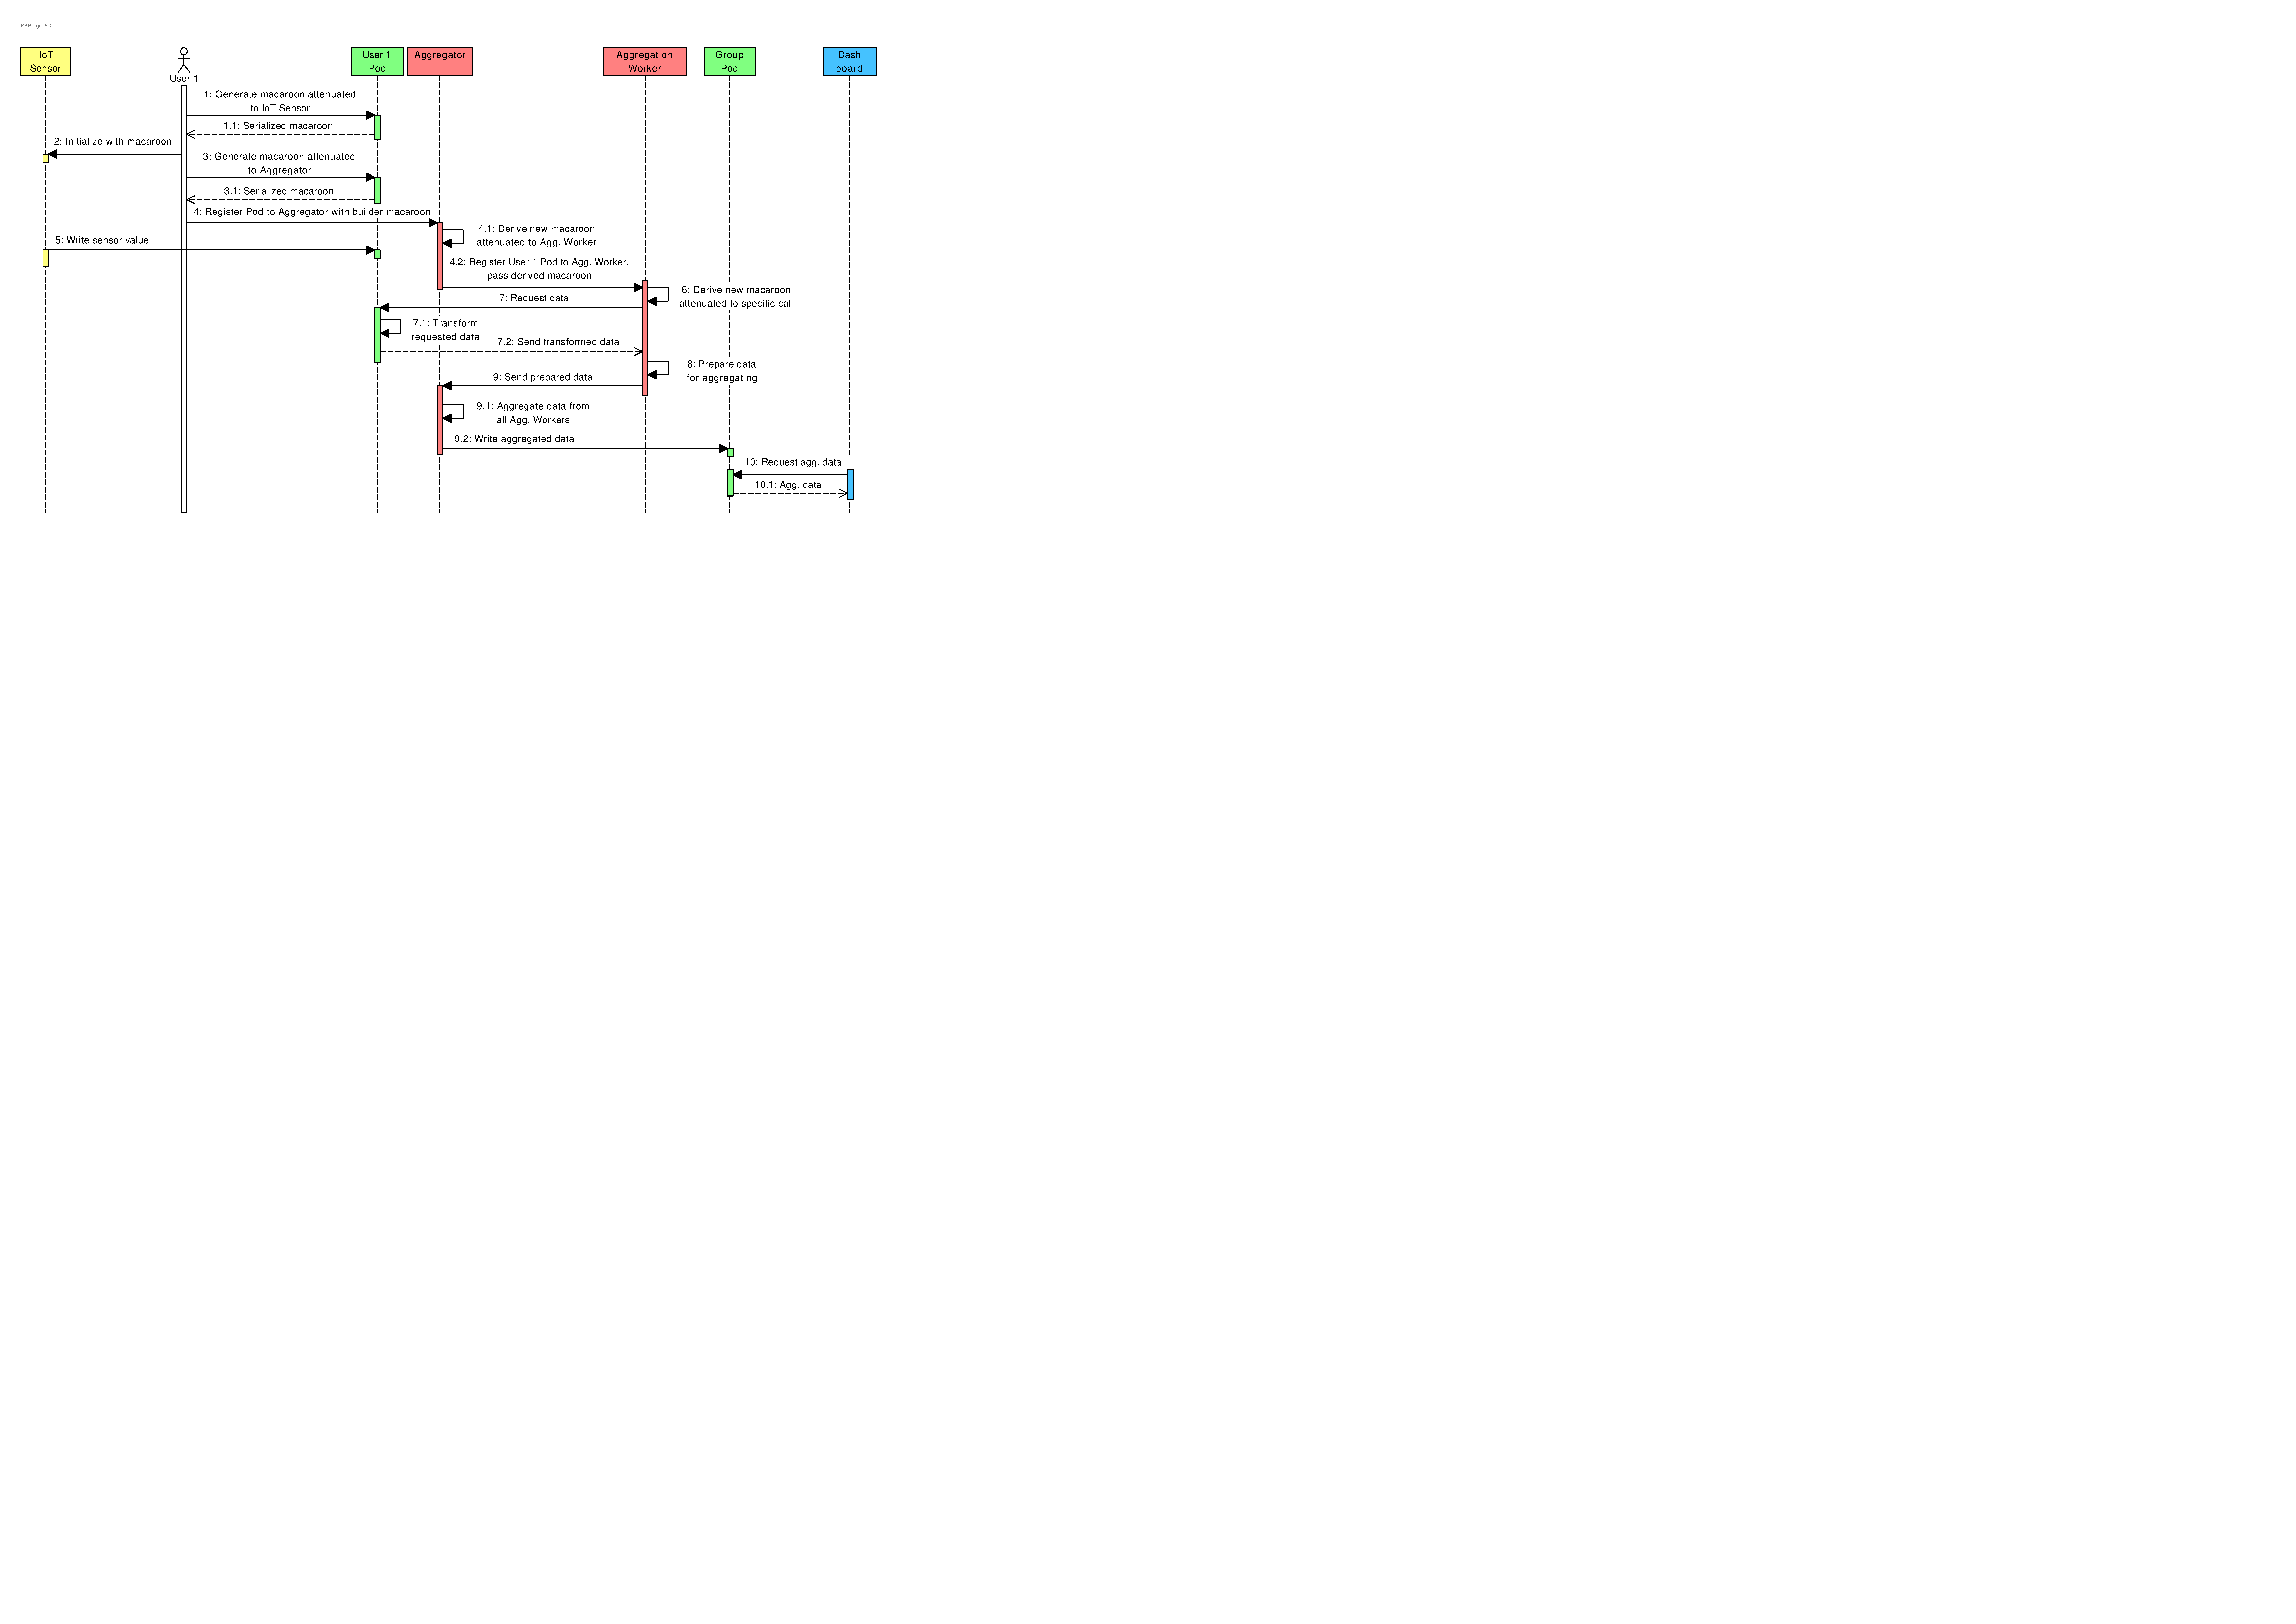
\includegraphics[width=1.0\textwidth]{images/architecture/InteractionDiagram-Aggregation-flow.pdf}
    \caption{Aggregation flow}
    \label{fig:aggregation-flow}
\end{sidewaysfigure}
